% Created 2013-05-10 Fri 22:50
\documentclass{article}
\usepackage[utf8]{inputenc}
\usepackage[T1]{fontenc}
\usepackage{fixltx2e}
\usepackage{graphicx}
\usepackage{longtable}
\usepackage{float}
\usepackage{wrapfig}
\usepackage{soul}
\usepackage{textcomp}
\usepackage{marvosym}
\usepackage{wasysym}
\usepackage{latexsym}
\usepackage{amssymb}
\usepackage{amstext}
\usepackage{hyperref}
\tolerance=1000
\usepackage{fontspec}
\usepackage{xunicode}
\usepackage{xltxtra}
\usepackage{xeCJK}
\usepackage{listings}
\usepackage{xcolor}
\usepackage{fancyhdr}
\usepackage{fancybox}
\usepackage{comment}
\usepackage{enumerate}
\usepackage{colortbl}
\usepackage{framed}
\usepackage{amsmath}
\usepackage{algorithm}
\usepackage{algorithmic}

\setmainfont{Times New Roman}
\setmonofont{Courier New}
\setCJKmainfont[BoldFont=YouYuan]{SimSun}
\setCJKfamilyfont{song}{SimSun}
\setCJKfamilyfont{msyh}{微软雅黑}
\setCJKfamilyfont{fs}{FangSong}

\lstset{frame=single}

% new and renew command
\newcommand{\reffig}[1]{Figure~\ref{#1}}
\newcommand{\reftbl}[1]{Table~\ref{#1}}
\renewcommand{\contentsname}{目录}
\renewcommand{\baselinestretch}{1.2}

% In case you need to adjust margins:
\topmargin=-0.0in      %
\evensidemargin=0.5in     %
\oddsidemargin=0.5in      %
\textwidth=5.5in        %
\textheight=8.5in       %
\headsep=0.25in         %
\author{计92 丘骏鹏 2009011282}
\date{2013-05-10}
\title{第十一周工作报告}
\hypersetup{
  pdfkeywords={},
  pdfsubject={},
  pdfcreator={Emacs 24.2.1 (Org mode 8.0.2)}}
\begin{document}

\maketitle

\section{本周工作}
\label{sec-1}
本周主要做的是检测重复记录(Data Record)工作
\subsection{具体实现}
\label{sec-1-1}
采用后缀树,实现了Ukkonen在1995年提出的一个\(O(n)\)的一个后缀树构建算法。(论文:
Ukkonen, Esko. "On-line construction of suffix trees." Algorithmica 14.3 (1995):
249-260.)。具体的描述挺复杂,参考了\href{http://stackoverflow.com/questions/9452701/ukkonens-suffix-tree-algorithm-in-plain-english}{Stackoverflow上面的一个解答} 及其补充进行实现。
(之前有搜索过一些Github,pastebin上面的开源代码,但是人工构造一些测例后发现我找
到的一些开源实现有bug,此外我们还需要根据本项目的需要修改代码实现,所以还是自己写
了一个)。

举一个html文件为例:
\begin{figure}[htb]
\centering
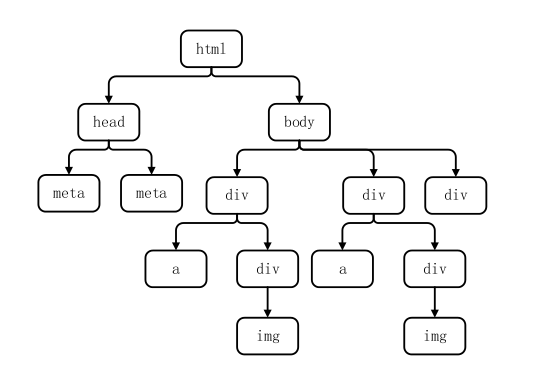
\includegraphics[width=0.8\textwidth]{./domtree.png}
\caption{\label{fig:1}DOM Tree}
\end{figure}

采用先序遍历,然后将 \texttt{<tag><tag/>} 标签对换成 \texttt{<tag+depth>} 标签加上深度的表示方
式,得到以下序列
\begin{verbatim}
html1 head2 meta3 meta3 body2 div3 a4 div4 img5
div3 a4 div4 img5 div3 a4 div4 img5 div3
\end{verbatim}

构造出一个后缀树为:
\begin{figure}[htb]
\centering
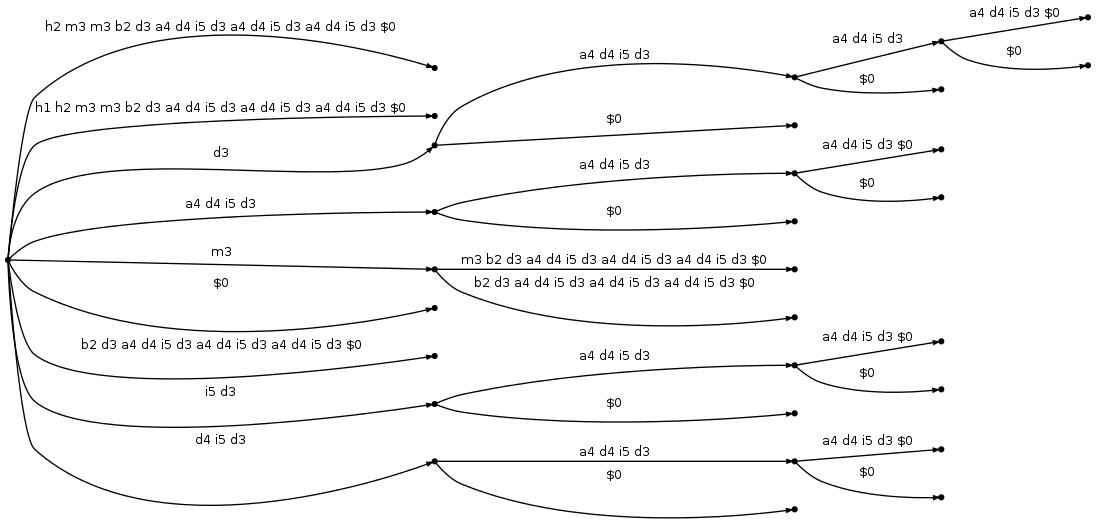
\includegraphics[width=\textwidth]{./tree.png}
\caption{\label{fig:2}Suffix Tree}
\end{figure}

注:为了能够在图片中显示完整,标签名做了简化

根据构造出的后缀树可以马上得到所有的重复序列及其在原序列中出现的次数,但是有以下
问题:
\begin{enumerate}
\item 重复序列的区间可能会相交
\item 重复序列的区间可能会有包含关系
\end{enumerate}

因为第一个问题的存在,由后缀树得到的公共序列不能直接使用。我们采用的是先序遍历的
方式,因此可以保证每个子树的所有标签序列位于一段连续的区间内。因此,可以在遍历后
缀树得到公共序列的时候人为“切断”一些公共序列,“切口”位于后一个标签的深度比前
一个标签的深度更大的地方(即两个子树的分隔点)。以上面的序列为例,遍历后缀树可以
得到所有的重复子序列为:
\begin{verbatim}
a4 div4 img5 div3
a4 div4 img5 div3 a4 div4 img5 div3
div4 img5 div3
div4 img5 div3 a4 div4 img5 div3
img5 div3
img5 div3 a4 div4 img5 div3
div3
div3 a4 div4 img5 div3
meta3
\end{verbatim}

改进以后公共的序列为:
\begin{verbatim}
a4 div4 img5
div4 img5
img5
div3
div3 a4 div4 img5
meta3
\end{verbatim}

这样就可以保证我们得到每个序列都是一个子树的一部分,这样就不会出现各个序列的区间
相交的情况。

为了解决子序列互相包含的情况(如"a4 div4 img5"和"div4 img5"),需要首先遍历后缀树,
得到所有的序列的区间,然后对所有的区间进行合并。普通的区间合并的做法会比较复杂,
需要借助其他数据结构,但是得到的这些公共序列有一些特点:不相交,且互相包含的区间
结束索引是一致的(即如果一个序列A包含序列B,序列B一定是A的某个后缀)。这样就可以
只需要扫描一遍所有的序列,利用Hash进行去重,然后合并所有的区间。

最后得到的公共的序列为:
\begin{verbatim}
div3 a4 div4 img5
meta3
\end{verbatim}

根据以上结果,对于每个重复出现的序列,去掉除了第一次出现的序列以外的所有的重复的
序列,原来的序列:
\begin{verbatim}
html1 head2 meta3 meta3 body2 div3 a4 div4 img5
div3 a4 div4 img5 div3 a4 div4 img5 div3
\end{verbatim}

可以简化为:
\begin{verbatim}
html1 head2 meta3 body2 div3 a4 div4 img5 div3
\end{verbatim}

从结果来看,基本完成了我们的目标。
\section{下一步工作}
\label{sec-2}
在网页数据上,目前只在小量的数据集上做过测试,还未完全利用到原有的框架中。从时间
上看,每个网页处理的时间需要0.2s左右,但是这些都只要离线处理,这个时间是可以接受
的。

这个周末开始准备做一些大一些规模的测试和模板提取的工作。
% Emacs 24.2.1 (Org mode 8.0.2)
\end{document}